\chapter{Implementation}
\label{chapter:Chapter 4}
\lhead{Chapter 4. \emph{Implementation}}

In this Chapter, we present a description of the Implementation of \todo[inline]{need a framework name}. Firstly, we provide a Data Analysis from the provided Historical data, which \todo[inline]{needs way more talk}.

\section{Data Analysis}
\label{section: Data Analysis}
In order to gain insight and find the limitations of the AIS Data, our initial step towards the implementation of the framework was a the analysis of an Historical AIS Data-Set. The analyzed Data-Set was compiled, and made publicly available by another H2020 European Project\footnote{http://datacron-project.eu}.  The choice of this Data-Set was done, due to the completeness of Documentation and Description of the actual Data-Set, which to the extend of our knowledge, was the only open-source Data-Set with this characteristics.  

Thus, in this Section, we present a Data Analysis made from the Data-Set\cite{DATASET}. The Analysis was done by firstly analyzing the overall distribution of the Data-Set and after the general analysis of each variable.  

The used Data-Set, is composed of \textbf{18.684.115} AIS Messages originated by \textbf{4555} different Vessels. The Data-Set covers a Period of 6 Months (from 2015-10-01 to 2016-03-31), from a area nearby Brest, France as it is presented in Figure \ref{fig:DS_Sample}.

\begin{figure}[H]
	\centering
	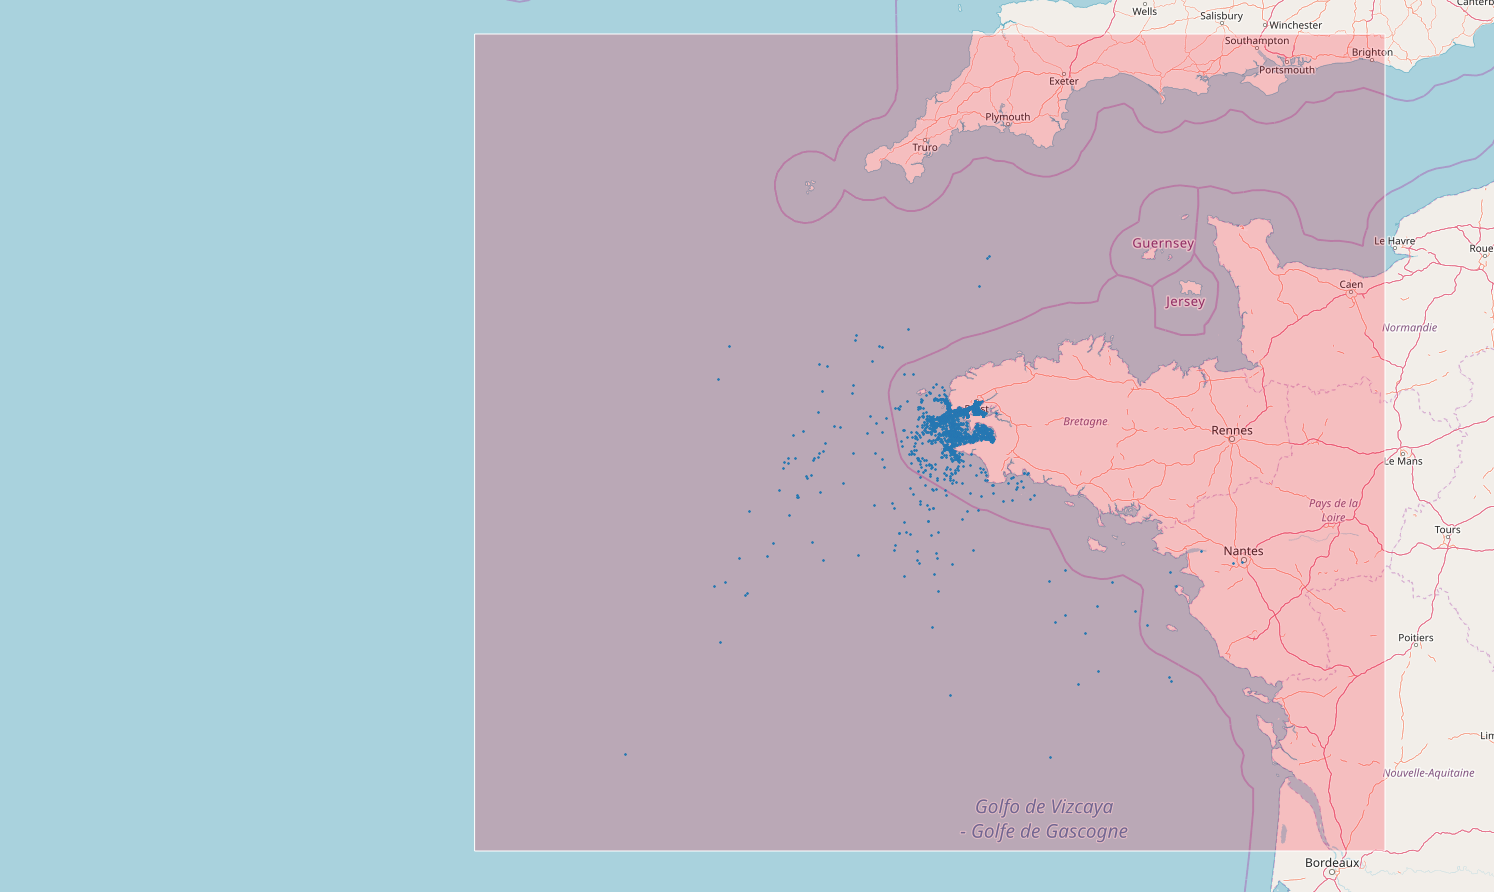
\includegraphics[scale = .23]{figures/Ch4/nari_DS_ex2.png}
    \caption{Area of the Data-Set represented in the Red, with a sample of 50.000 AIS Positions.}
    \label{fig:DS_Sample}
\end{figure}

Every AIS Message provided in the Data-Set, is composed by the features that derive from the AIS Dynamic Information. In Table \ref{Table: Data-Set Features}, we describe the Data-Set features and also the unit and range of each feature. 

\begin{table}[H]
\centering
\caption{AIS dynamic messages features description.}
\label{Table: Data-Set Features}
\begin{tabular}{@{}llll@{}}
\toprule
Feature & Description                  & Unit               & Range          \\ \midrule
MMSI    & Vessel Unique Identifier.     &                    & 0 to 99999     \\
Status  & AIS Navigational Status.     &                    & 0 to 15        \\
Turn    & Rate of turn, right or left. & degrees per minute & 0 to 720       \\
SOG     & Speed Over Ground.           & knots              & 0 to 111*      \\
COG     & Course Over Ground.          & degrees            & 0º to 360º     \\
X       & Longitude.                   & degrees            & -180º to +180º \\
Y       & Latitude.                    & degrees            & -90º to 90º    \\
Time    & Received Time-Stamp.         & Unix Time          &                \\ \bottomrule
\end{tabular}
\end{table}

The Data-Set contains not only the Dynamic information correspondent of the AIS messages, but also the related Vessel Static Information of each Vessel from the Data-Set. By interpolating the MMSI reported in every AIS message, we were able to enrich each dynamic message, with the static information related to the Vessel which produced this message. The Vessels Static Information correspond to the actual Vessels dimensions and Type. The use of this information related to the Vessels characteristics is used in different types of Behavioural Analysis. In this work we used the Vessel Type as an aggregation indicator, which is better described in Section \ref{subsection: Vessel Type}.

\section{Implemented Framework}
\todo[inline]{need to intro the framework talk about the used techinques. -> kafka -> spark?!? -> cassandra}

\section{Data Ingestion}
\todo[inline]{}
Data Ingestion refers to the model, where the Data is input into the Framework. As mentioned in Chapter III, was assumed for this work that data would be able to come in two different typologies, either from Batches of Data or Live NMEA streams. 

The Framework was developed to be scalable, being able to handle different sources of AIS data, although for the purpose of this work, we limited the used Data to two main sources of Data. The Data-Set presented in Section \ref{section: Data Analysis}, and the NMEA feeds made available by the Portuguese Navy.




\section{Data Pre-processing}
Data Pre-processing, represents the module that handles the Raw AIS data, Cleaning, Transforms and Normalizes every AIS messages, coming from the Data Ingestion Module. Every AIS message is transformed into our normalized representation of and AIS message, which we defined as a \textbf{Behavioural Point}, defined under in \ref{subsection: Behavioural Point}.

\subsection{Latitude Longitude Normalization}
In order to normalize the reported AIS positions, either from the AIS streams or the used Data-Set, we defined a set number of decimal cases used. This is done as most of AIS providers only assure a GPS precision of 0.0001 minutes accuracy, but what we found was that some reported positions come with up to 8 decimal cases, which can be caused just from how the Data-Set files were written.

So our normalization process, was to assure that every Vessel position was normalized to a precision on 4 decimal cases; as it represents a global position precision of 11m to 4m, as it is shown in Table \ref{Table: Degree Precision}.

\begin{table}[H]
\centering
\caption{Degree precision versus the approximate radius of measured error.}
\label{Table: Degree Precision}
\begin{tabular}{lrrrr}
\hline
\multicolumn{1}{c}{\begin{tabular}[c]{@{}c@{}}Decimal \\ Places\end{tabular}} & \multicolumn{1}{c}{Degrees} & \multicolumn{1}{c}{\begin{tabular}[c]{@{}c@{}}Precision \\ Equator\end{tabular}} & \multicolumn{1}{c}{\begin{tabular}[c]{@{}c@{}}Precision \\ 45º N/S\end{tabular}} & \multicolumn{1}{c}{\begin{tabular}[c]{@{}c@{}}Precision \\ 67º N/S\end{tabular}} \\ \hline
0 & 1.0 & 111.3Km & 78.7Km & 43.5Km \\
1 & 0.1 & 11.3Km & 7.8Km & 4.4Km \\
2 & 0.01 & 1.13Km & 787.1m & 435m \\
3 & 0.001 & 111.3m & 78.7m & 43.5m \\
4 & 0.0001 & 11.3m & 7.8m & 4.4m \\
5 & 0.00001 & 1.3m & 0.7m & 0.4m \\ \hline
\end{tabular}
\end{table}
\todo[inline]{Geohash - https://en.wikipedia.org/wiki/Geohash}
\todo[inline]{Another techniques?!?}

\subsection{Data Cleansing}
Data Cleaning refers to the process of cleaning the Data which is wrongly defined or, has wrong types. When handling with sensor Data that is transmitted is common that wrong readings occur. In AIS data, this errors tend to occur as AIS features that are not transmitted with values that don't correspond to the Feature value range. An example of this is having a Latitude being broadcast with values of 500.
\todo[inline]{maybe a table with the limits of each variable}
For the messages transmitted with features that didn't correspond to the value range of the specific Feature, we discarded this messages. The features value range considered for the whole framework was the one presented in \ref{Table: Data-Set Features}.

\subsection{Behavioural Point}
\label{subsection: Behavioural Point}
A Behavioural Point is a multidimensional point $BP_{MMSI}$ is defined as:
\[BP_{MMSI} = [t, x, y, SoG, CoG, NS]\]
Where the dimensions of the multidimensional Behavioural Point represents the (Time, Longitude, Latitude, Speed Over Ground, Course Over Ground and Navigational Status) respectively, a representation of these features is provided in Table\ref{Table: Data-Set Features}. The Maritime Mobile Service Identity (MMSI) representing a unique identifier of each Vessel, was used for this work as the identifier of each $BP_{MMSI}$, we assumed the non replication of this identifier on different Vessels would occur.

using this Identifier to and the MMSI represents the Unique Identifier of the Vessel.



\section{Feature Engineering}
\subsection{Vessel Type}
\label{subsection: Vessel Type}
Vessel Type, is a classification system, where each Vessel is categorized by the type of activities it preforms. Classified by a numeric scale from 0 to 99; the first digit represents the general category of the subject Vessel, and the combination of the first digit with the second represent a specific activity of the Vessel. In Table XX we present the Vessel General category associated with the first digit, and also the specific Categories which are more representative in the Data-Set.

\begin{table}[H]
\centering
\caption{My caption}
\label{my-label}
\begin{tabular}{@{}llll@{}}
\toprule
First Digit & General Category & Relevant Categories &                                                                                         \\ \midrule
1           & Reserved         &                     &                                                                                         \\
2           & Wing In Ground   &                     &                                                                                         \\
3           & Special Category & 30 - Fishing        & 30 - 286(6\%)                                                                           \\
4           & High-Speed Craft &                     &                                                                                         \\
5           & Special Category &                     &                                                                                         \\
6           & Passenger        &                     &                                                                                         \\
7           & Cargo            & 70 - Cargo          & \begin{tabular}[c]{@{}l@{}}70 - 1511(33\%)\\ 79 - 273(6\%)\\ 71 - 217(5\%)\end{tabular} \\
8           & Tanker           & 80 - Tanker         & 80 - 342(7\%)                                                                           \\
9           & Other            &                     & 99 - 1192(26\%)                                                                         \\ \bottomrule
\end{tabular}
\end{table}

For the usd Data-Set described above in Section\ref{section: Data Analysis}, the Static Vessel Information is available for all the Vessel in the Data-Set. Although, when handling Real-Time NMEA streams or other Batches of Data, the Vessel Static information is not available or broadcast. This, creates a problem of not having the Vessel Type information which is used to query our Trajectory Data-Base.
For this we developed a \textbf{Web Scrapping application}, described in the following subsection.

\subsubsection{Vessel Type Scrapper}
Web Scrapping is used to extract information from freely available websites. For the sole purpose of this work, we developed an application that would retrieve the Vessel Type information from a well Known Vessel Traffic Webpage.
By giving a Vessel Identifier (MMSI) to the Vessel Type Scrapper, we retrieve the html webpage data that contains all the Vessel Information from the well Known Vessel Traffic Webpage. From the html data we, strip the html tags thus retrieving the Vessel Type Information, as it is presented in Fig. \ref{fig:Scraper}.

\begin{figure}[H]
	\centering
	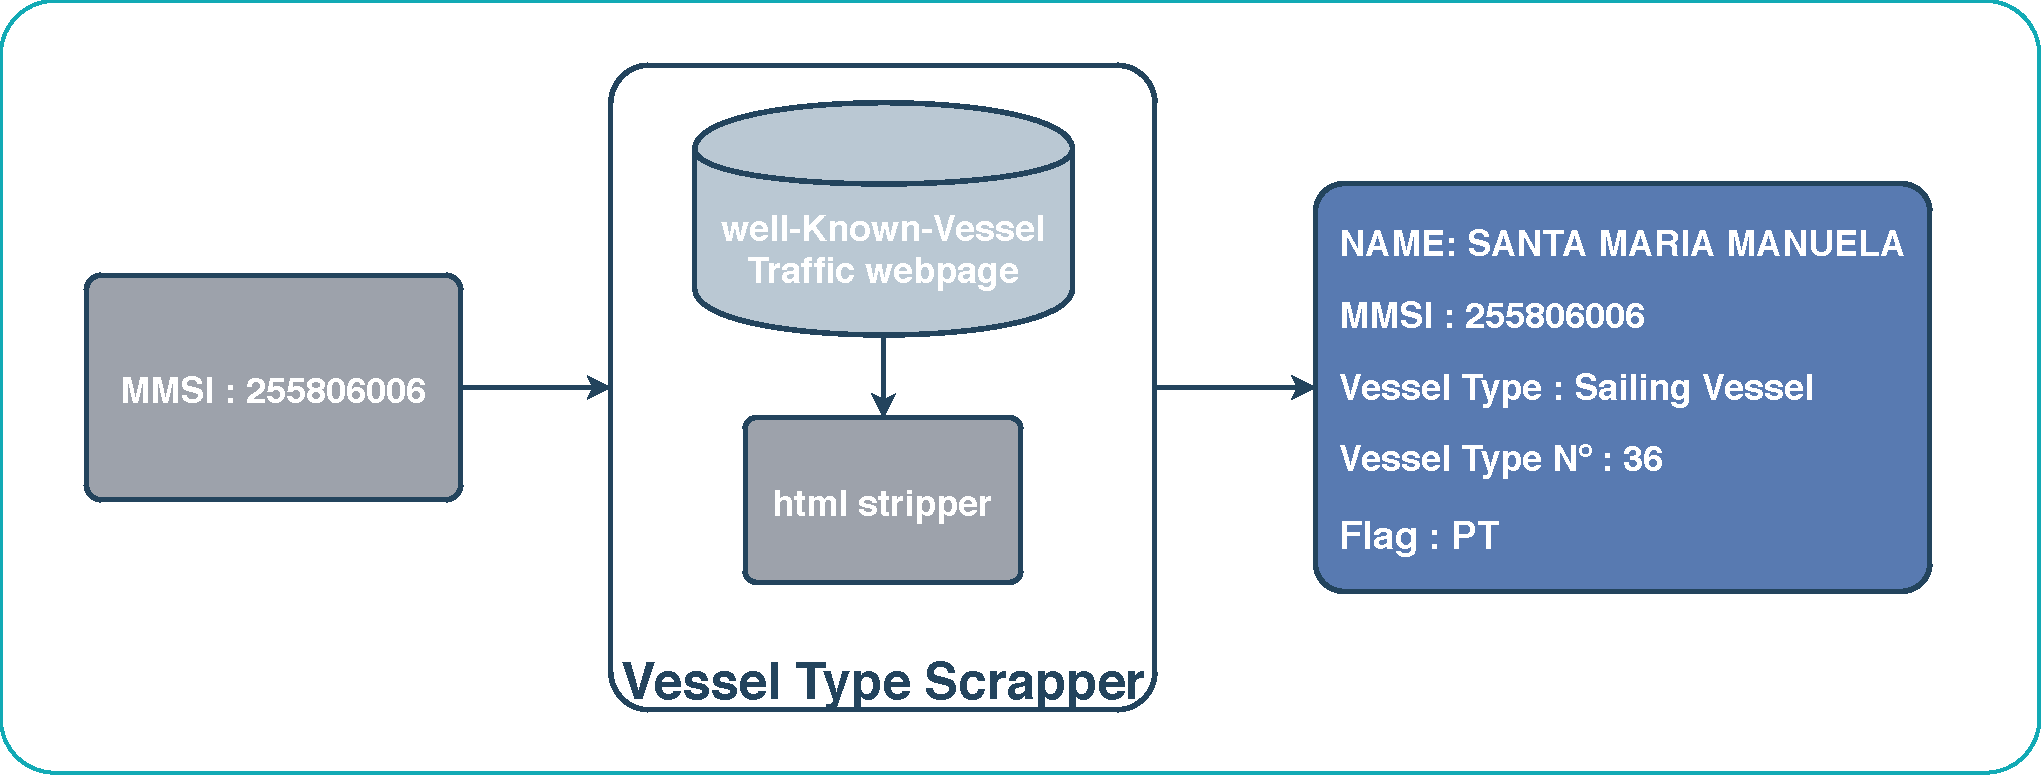
\includegraphics[scale = .4]{figures/Ch4/scrapper}
    \caption{Example of the Vessel Type Scrapper retreived information for Vessel MMSI: 255806006}
    \label{fig:Scraper}
\end{figure}


\subsection{Distance to Coast}
The Distance to Shore influences, the navigational behaviour for some type of Vessels. In order to enrich the features used in our Anomaly Detection methods it seemed necessary to extrapolate the Distance to Shore for every point in the Data-Set. Although in order to calculate the Distance to Shore over the whole data-set, and in real time to streams of AIS data it is mandatory to represent the Coastline in a efficient manner. 
For this we used the ocean coastline data\footnote{http://naturalearthdata.com}, which represented the Global Ocean Coast line in a vector of \textbf{547.503} points, which is equivalent of representing in a 1:10m scale.

The calculation of the closest point was done with a Nearest Neighbor approach, using the Ball Tree algorithm. The choice of this algorithm was done, due to the high volume of data we were using, and the possibility of using the Haversine Distance measures \eqref{eq: Haversine} in the already implemented methods from \footnote{http://scikit-learn.org/stable/modules/generated/sklearn.neighbors.BallTree.html}.

Haversine is a distance metric commonly used in Vessel Navigation, as both Latitude and Longitude features are represented in a spherical coordinate system. $d_({p_1}, {p_2})$ represents the distance between the 2 point $p1(lat_1, lon_1)$ and $p2(lat_2, lon_2)$, and where $r$ represents the approximate radius of the Earth which we considered \textbf{6.367.000m} in our experiments.

\begin{equation}
d = 2r sin ^{-1} (\sqrt{sin^2(\frac{lat_{2}-lat_{1}}{2})+cos(lat_{1})cos(lat_{2})sin^2(\frac{long_{2}-long_{1}}{2}))}
\label{eq: Haversine}
\end{equation}

\subsubsection{Distance to Port}
Distance to Port, represents a feature that can be used in many ways such as  analyzing a Vessel Behaviour, or one that actual represents a great importance to Maritime International Trade, estimating the Vessel Time of Arrival,  \cite{Moussa2018ScalableSpark}, \cite{Rosca2018PredictingRoutes}.
 
We then enriched each $Behaviour Point$ by calculating, what was the nearest Port, and what distance it was. This was done, based on the same Methodology presented in Section above. 

Although, getting a list of every port was not trivial, as there are numerous Ports around the World, and such information is not 
centralized nor normalized.
We accesed the detailed information of the World Port Indexes in \footnote{http://msi.nga.mil/MSISiteContent/StaticFiles/NAV\char`_PUBS/WPI}. The World Port Index data was in a GIS(Geographic Information System) shapefile format, which is common format for the Maritime Domain, but not usable in our Framework, thus we firstly normalized the data format using the Python Package dbfread \footnote{http://dbfread.readthedocs.io}, and storeded the normalized data in our Data-Base. 
For each of the \textbf{3865} ports we extrated the respective Port position, Country, and Name. 
In Fig. we present the position of the ports of the Iberian coast in Orange.

\begin{figure}[H]
	\centering
	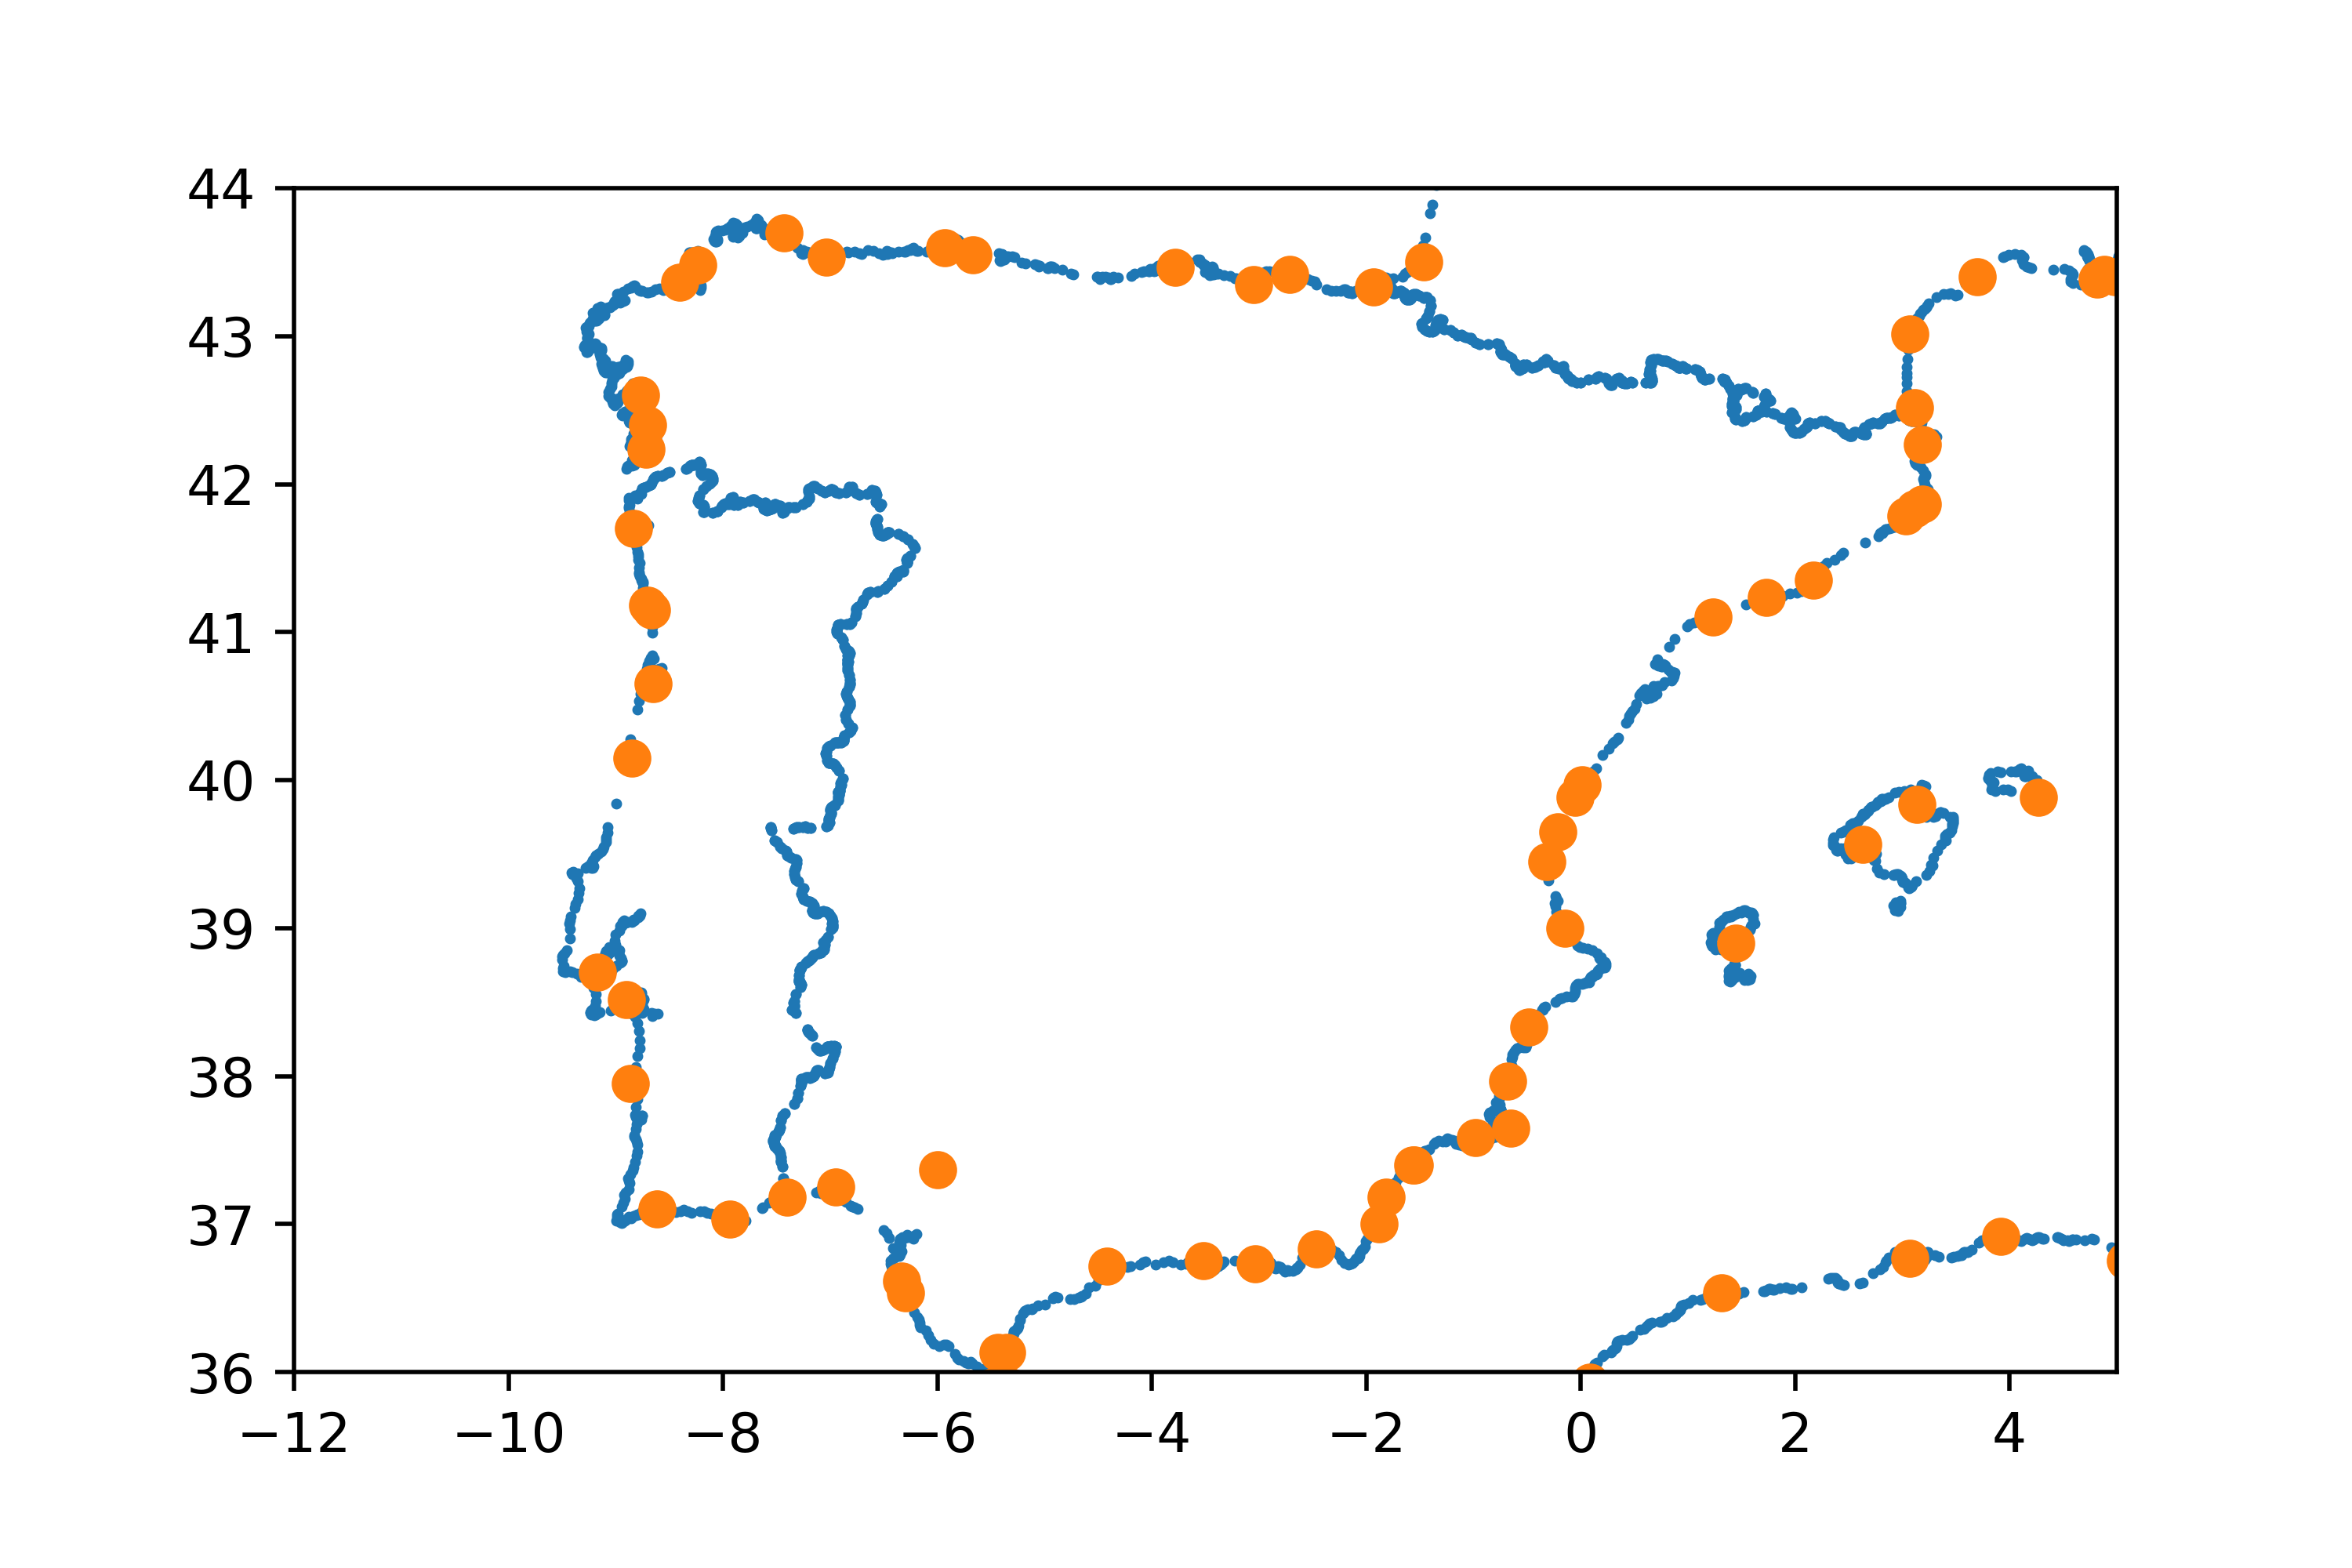
\includegraphics[scale = .9]{figures/Ch4/ports.png}
    \caption{}
    \label{fig:asdsadsadasda}
\end{figure}


\subsection{Stopped/Moving}
\label{subsection: Stopped/Moving}
Enriching the reported Vessel Kinematics by determining if whether a Vessel is Moving or Stopped represents a information gain on overall Vessel Trajectory that can be addressed, for the understanding of the normal Vessels Behaviour itself and even further, the possible detection of Anomalies.
Thus, the approaches we used to classify every Vessel transmission as Stopped or Moving is shown in the following subsections:

\textbf{Rule Based Approach}:
This approach is vastly used in the literature, as it is the simplest way to characterize the stopping of a Vessel, based solely on the Speed or as reported in the AIS the Speed Over Ground (SOG). Thus, Vessels Positions that have a Speed under a certain defined threshold $\Delta$ are considered as Stopped and the opposite are considered Moving, as it is shown in equation \ref{eq: MovingRule}, where $p_n$ represents actual point we want to the point which we want to c.
\begin{equation}
kinematic status(p_n) = \left\{\begin{matrix}
p_n.SOG > \Delta; & Moving\\ 
p_n.SOG \leq  \Delta; & Stopped
\end{matrix}\right.
\label{eq: MovingRule}
\end{equation}

The most commonly used value, found in the literature for $\Delta$ was 0.5 knots, which was also the Threshold we initially tested for, but we found that this leads to the miss-labeling of effectively Positions that are Moving, more specifically Fishing Vessels that due to their type of fishing activities, greatly slow their Speed for short periods of Time, which cannot be labeled as Stopped.
\todo[inline]{Need intro to this image, Trajectory of a Shipping Vessel that is considered as stopped. just painting point by point}
\todo[inline]{Need new Image too...}

\begin{figure}[H]
	\centering
	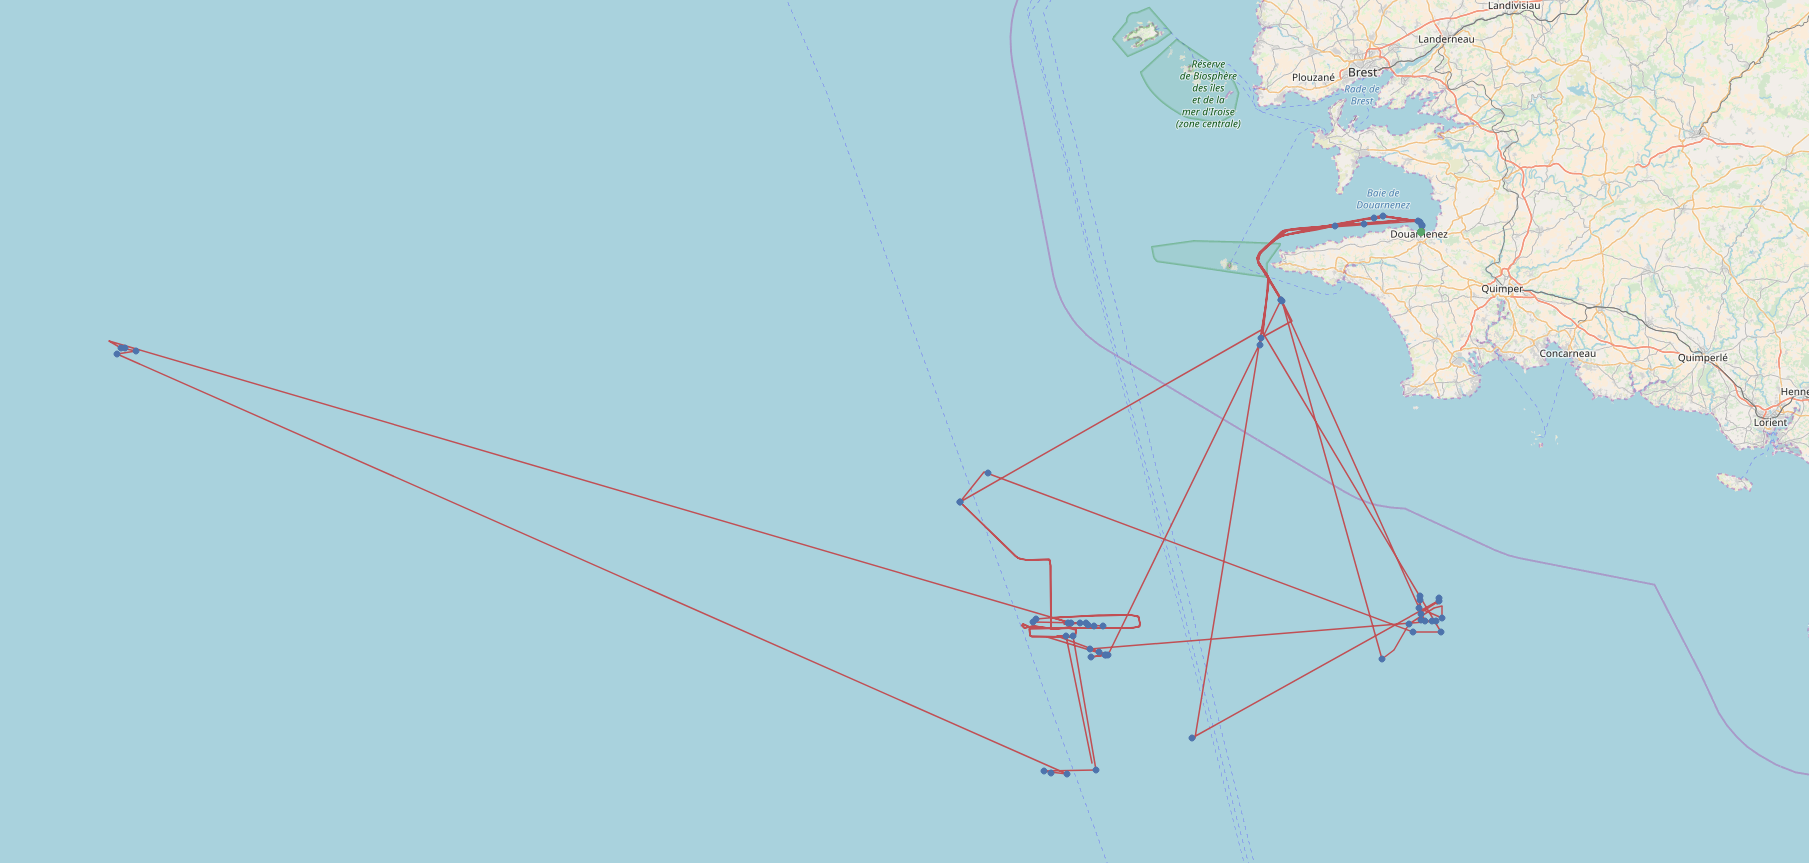
\includegraphics[scale = 0.15]{figures/Ch4/simplestopMoving228858000.png}
    \caption{Vessel 228858000}
    \label{fig: 228858000}
\end{figure}

\section{Unsupervised Trajectory Extraction}
In this Section we present our definition our interpretation and formulation of Vessel Trajectory, 

\subsection{Trajectory Definition}
Representing a Vessel Trajectory data, can become a difficulty in the Maritime domain. Currently there are a vast number of solutions described in the literature, presenting different solutions for different types of problems. 

Our approach to represent a Maritime trajectory, was to consider a trajectory as a whole, this is, as Vessel are obliged to broadcast their AIS information in a semi-continuous rates; by defining a \textbf{Behavioural Point} to each received AIS message, we can aggregate every BP based on the Vessel identifier of each Vessel, thus representing Trajectory as a set BP, represented as 
\[TR_{MMSI} = BP_{MMSI_1}, BP_{MMSI_2}, BP_{MMSI_3}, BP_{MMSI_4}, \cdots , BP_{MMSI_n}\]

We sort every Trajectory based on the Time-Stamp of each $BP_MMSI$, which allows us to consider a Trajectory into a Multivariate Time-Series. For each Trajectory we have $N$ time-series, in which $N$ represents the number of features considered for each trajectory which is similar to say that is the same number of features each BP has. further explained in the subsections bellow.

%knowing that each AIS broadcast message represent the instantaneous kinematic information from a Single Vessel, aggregating this information over time will represent a Vessel Trajectory. 

%Thus, by identifying each vessel by its unique identifier (MMSI), the trajectory can be considered as the set of AIS messages, identified by the MMSI of each Vessel.


%Although, as each AIS message is time-stamped(contains the time in which was broadcast), our representation of trajectory can be defined as 

\subsection{Multivariate Time-Series Analogy}
As mentioned above, each Trajectory is considered as a Time Series composed of Multiple features.  


\begin{figure}[H]
	\centering
	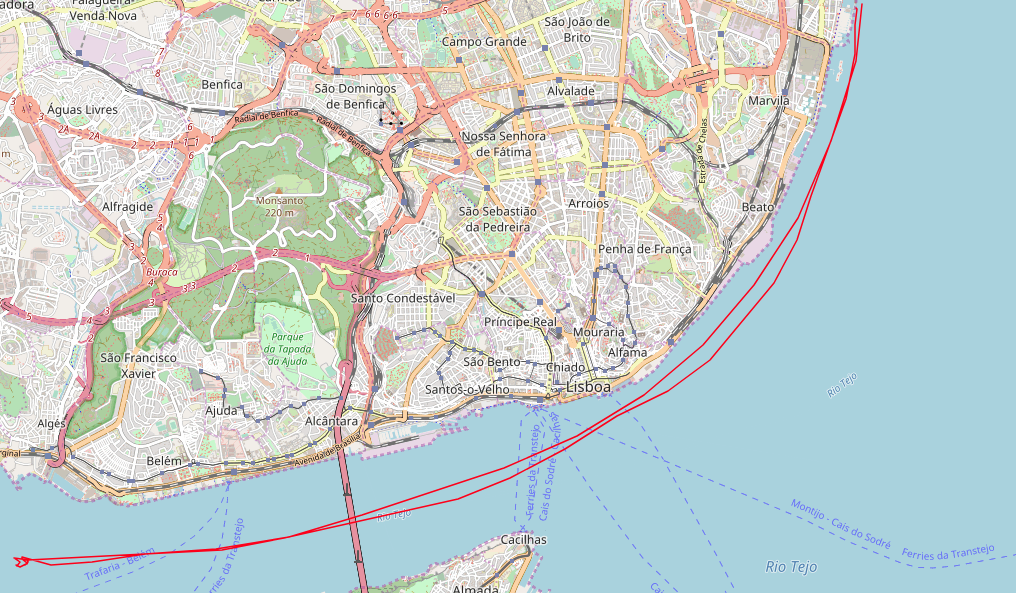
\includegraphics[scale = .3]{figures/Ch3/traj_example.png}
    \caption{Trajectory snapshot(2017-11-05 10:22 to 2017-11-05 22:42) from Vessel MMSI: 255806006}
    \label{fig: TrajectorySMM_example}
\end{figure}


in Fig. \ref{fig: MTimeSeries_example}, we represent the Vessel trajectory showend in figure X. 
For each trajectory we consider the features representing 
main features that a which in order to normalize our analysis of a Vessel Route, we ...
\todo[inline]{TODO dar palha para introduzir esta imagem}

\begin{figure}[H]
	\centering
	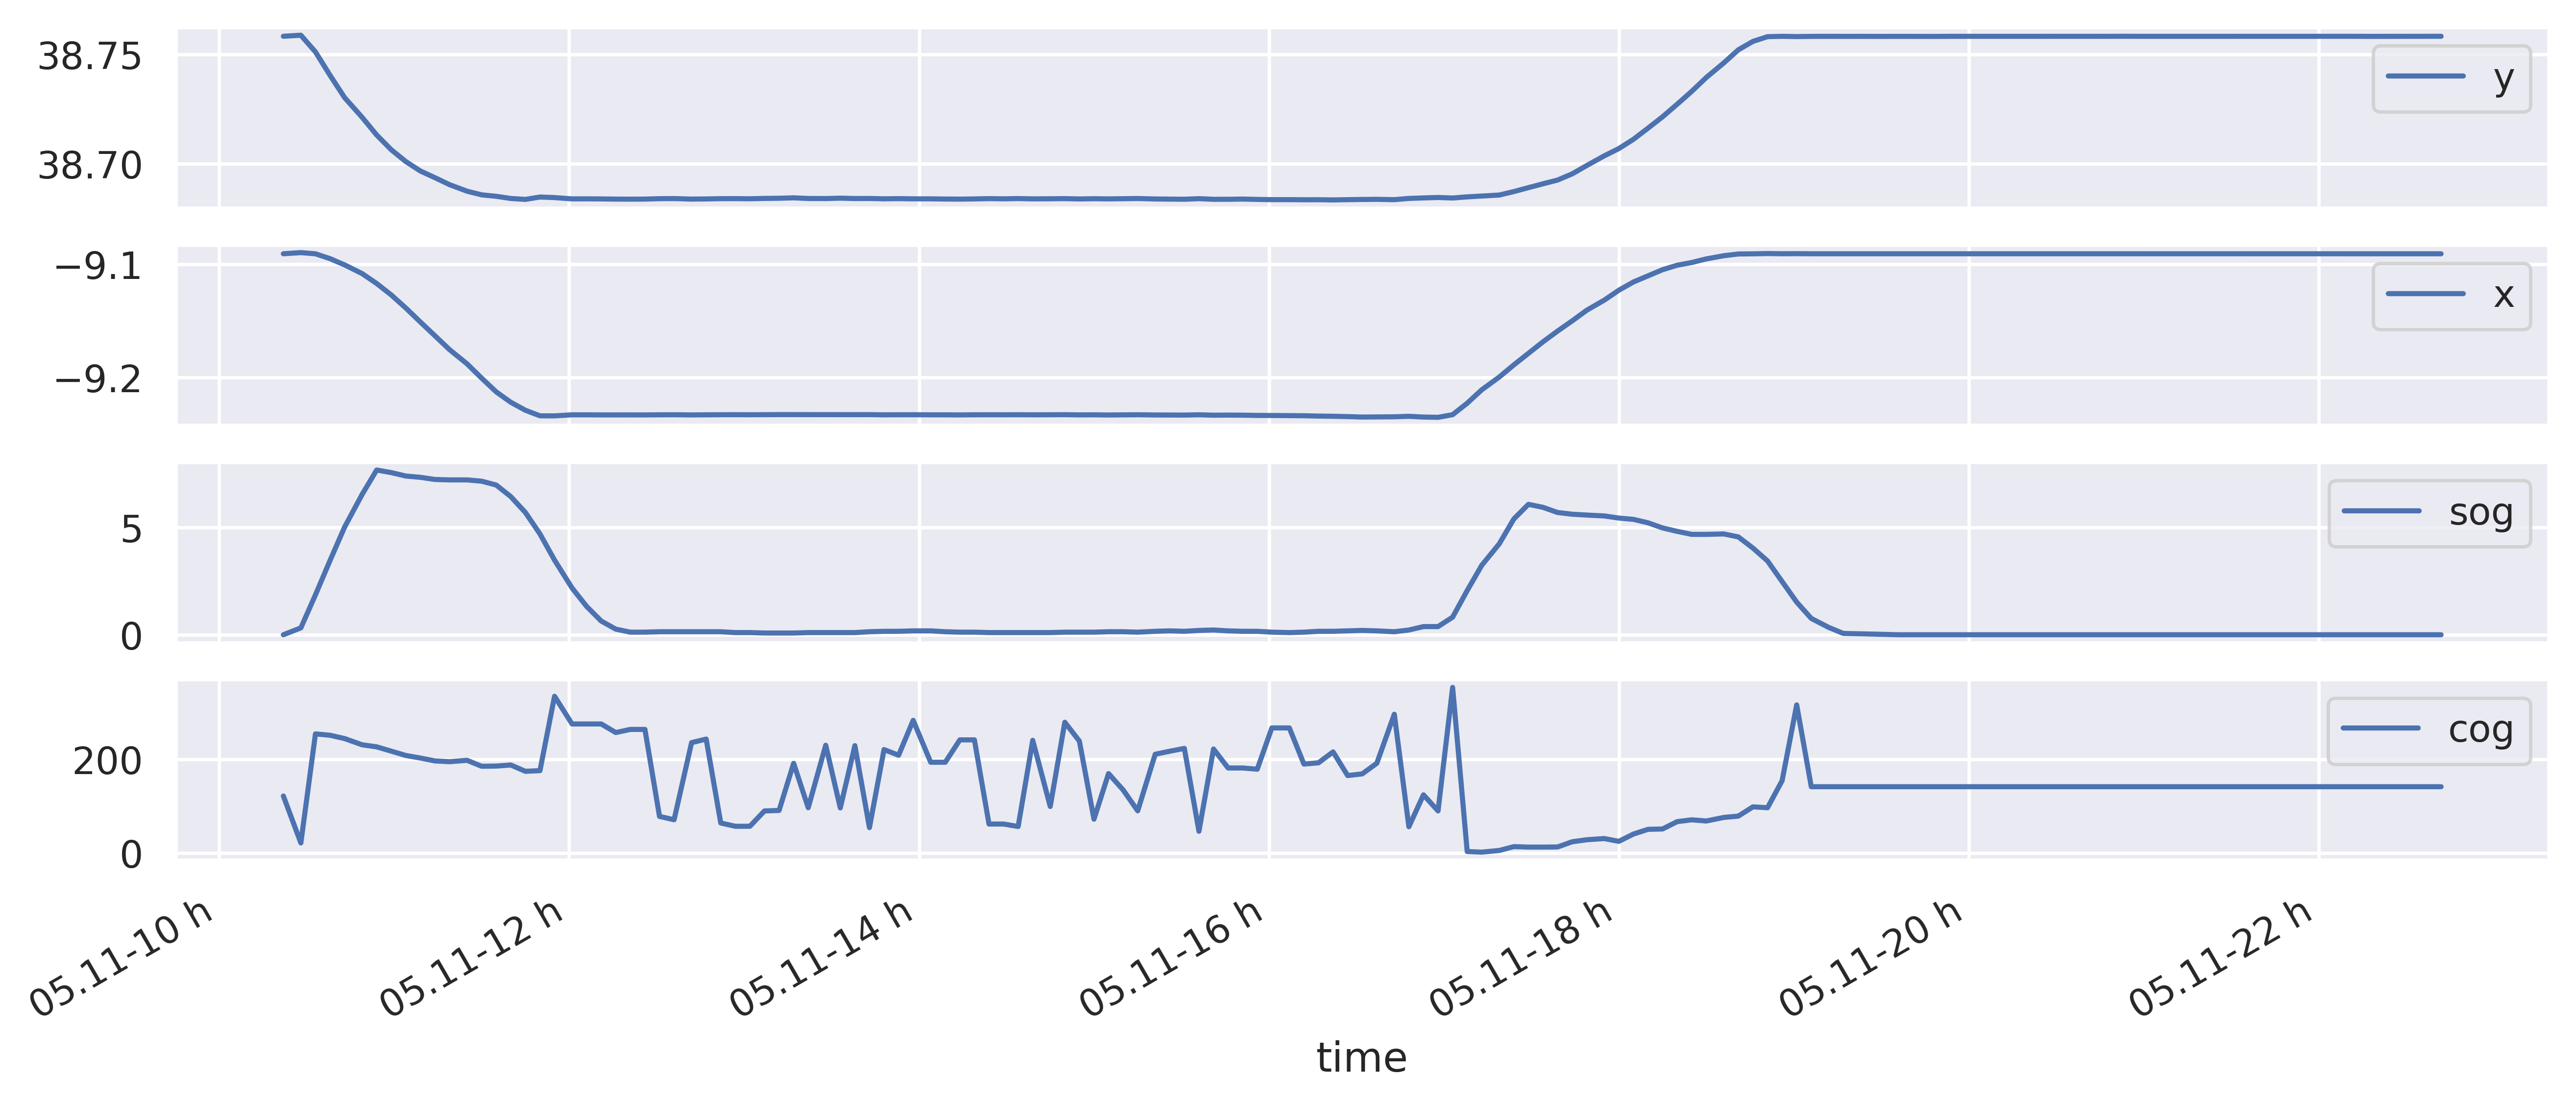
\includegraphics[scale = .5]{figures/Ch3/ts_example.png}
    \caption{Trajectory represented in Fig.X, presented as a Multivariate Time Series.}
    \label{fig: MTimeSeries_example}
\end{figure}

\todo[inline]{Needs Intro for this section...}

\subsection{Smoothed Stopped / Moving}
\label{subsection: Smoothed Stopped / Moving}
\todo[inline]{TALK ABOUT THE feature}

In order to mitigate the problem described in Section \ref{subsection: Stopped/Moving} we used a smoothing technique \textbf{Rolling Mean}, which is a common method used in Time Series Analysis. 
By Smoothing the Vessels $SoG$, based on the previous BP of each Vessel we reduce the random or abrupt variations in the observed Speed features, which ultimately leads to a better representation of the Vessels Kinematics.
\todo[inline]{Need intro to this image}

\missingfigure{Trajectory of a Shipping Vessel that is considered as stopped then with the rolling mean!}

\subsection{Time-Space Incompatibility}
Time Space incompatible corresponds to an anomalous or incoherent situation where the reported actual Vessels position is not compatible if compared with previous reported positions, and Vessels Kinematics. The detection of this situation, is also represented as an Anomaly Requirement ($AR_4$), in Section\ref{section: Framework Requirements}.

In order to detect this incoherence's, we developed a Method that takes as input an historical Vessels Trajectory $TR_{MMSI}$, and for each Behavioural Point ${BP_{MMSI}}^{T-1}$ we estimate the position of the Vessel at instance ${BP_{MMSI}}^{T}$.
The estimation is done by assuming that a Vessels Movement can be represented in a \textbf{Linear Motion}, as most of the Vessels tend to move in the most economical way, thus the Vessels traveled distance, can be calculated, using the formula :
\begin{equation}
Distance = Velocity . \Delta Time
\label{eq: dvt}
\end{equation}
Where $\Delta Time$ represents the actual Time Shift from point $(T-1)$ to $(T)$.

By calculating the equation \ref{eq: dvt} for each $BP^{T}$ based on the reported Position of the previous $BP^{T-1}$, we can predict that Vessel should be in a distance radius of $D$ for the next $BP^T$, as it is shown in Figure \ref{fig: dvt}.

\begin{figure}[H]
	\centering
	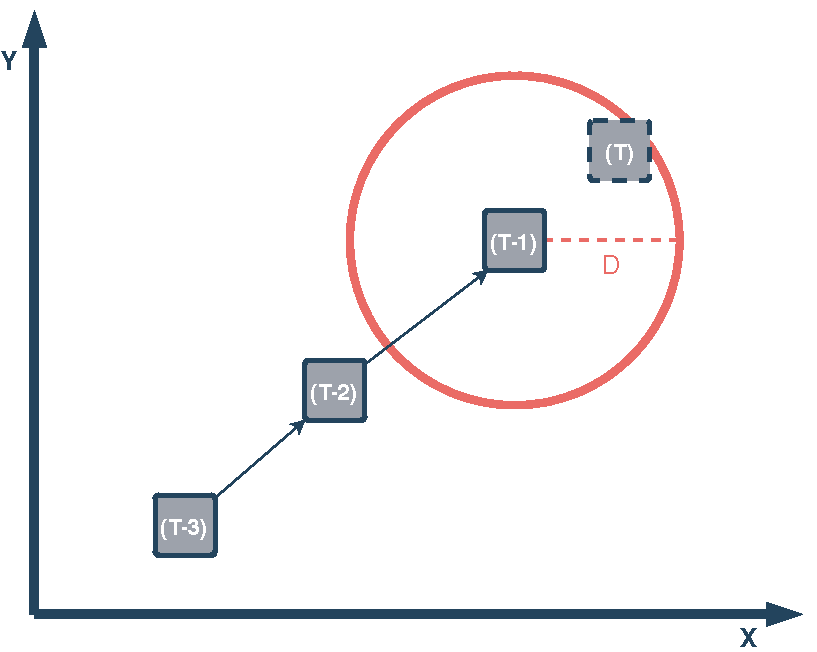
\includegraphics[scale = .6]{figures/Ch4/DVT.pdf}
    \caption{Linear Estimation}
    \label{fig: dvt}
\end{figure}

By defining a configurable Distance Factor Threshold $dft$, representing a factor that would be multiplied by $D$, is possible to deduct that, if the a Vessel at Time $BP^{T}$ is at a distance superior than $(D.dft)$, it is considered at a incoherent position, thus it is reported as Anomalous.

The emphasis of this Section was on the detection of Time-Space Incompatibly, which is achieved using the methods above. Although by assuming that Vessels have a huge inertia, making them unable to perform quick changes of not only speed but also direction, the authors in \cite{Sadowski2015AlgorithmsCompression} present a \textbf{Linear Estimation Algorithm}.
As the reported $CoG$ represents the direction of movement, it is possible to Equation \ref{eq: dvt}, thus estimating the actual position of the Vessel, opposed to the Distance from previous Position. 

\iffalse

the enfacis was on the  allowing the End-User to configure the $dft$ the granularity of the Incoherence Position reporting will be changed. And for this work we fo

representative of what a Vessel would travel based on the reported characteristics, based on a representing we can excan assume that defining a Distance Threshold,

the simple based on a Linear estimation of the Vessels Kinematics, which is similar 
The detection of this situation for our Framework, is used for two main objectives, the detection of the anomaly itself, and for the partitioning of Trajectories which is explain under in Section XX.
\fi




\section{Anomaly Detection Service}

\subsection{Navigational Status Validation}
AIS Navigational Status describes the Vessel current navigational activity based on a set static set of defined Status, as shown in Table XX. The Navigational Status needs to be manually set, and constantly updated (according to the current Vessel activity), by the Vessel crew members. 
The problem with relying on Human action to update the actual Vessel Navigational Status is that is really prone to errors. 

\begin{table}[H]
\centering
\caption{AIS Navigational Status enumeration.}
\label{Table: AIS Status}
\begin{tabular}{@{}cl@{}}
\toprule
\begin{tabular}[c]{@{}c@{}}Navigational \\ Status Value\end{tabular} & \multicolumn{1}{c}{Description} \\ \midrule
0 & under way using engine \\
1 & at anchor \\
2 & not under command \\
3 & restricted maneuverability \\
4 & constrained by draught \\
5 & moored \\
6 & aground \\
7 & engaged in fishing \\
8 & under way sailing \\
9 - 14 & reserved for future use \\
15 & Default \\ \bottomrule
\end{tabular}
\end{table}

The use of the wrong Navigational Status being considered an Anomaly, $(AR_4)$, our approach towards the detection of this Anomaly, started by firstly analyzing the use and the frequency of each Navigational Status. 

We concluded, based on the frequency count of each Status that there are AIS Status which are solely used in special scenarios. Thus, for this work we focus on the detection and validation of AIS Status that can be justified on the Vessels Dynamic Features.

\missingfigure{COUNT PLOT - AIS STATUS COUNTS}

With the help of Maritime Officers Expertise, we enriched our Description from each Navigational Status, be classifying the appropriate \textbf{Stopped or Moving Label} to each Navigational Status. Maritime Experts, based on what the Navigational Status Kinematics should represent provided the following
Table\ref{Table: AIS Status Moving or Stopped}.

\begin{table}[H]
\centering
\caption{My caption}
\label{Table: AIS Status Moving or Stopped}
\begin{tabular}{lc}
\hline
Expert Label     & Navigational Status Number \\ \hline
Stopped          & 1, 5, 6                    \\
Moving           & 0, 7*, 8                   \\
Non-Quantifiable & 2, 3, 4, 15                \\ \hline
\end{tabular}
\end{table}
$7^*$(the Engaged at Fishing) represents a Special Navigational Status which cannot be validated by a Stopped or Moving Analysis. The Validation of this specific Status is done in Subsection under, Section \ref{subsection: Fishing Activity Detection}.

The actual Navigational Status Validation, is done as a Point Based Comparison. By comparing the enriched Feature\textit{Smoothed Stopped or Moving}(Section \ref{subsection: Smoothed Stopped / Moving}) with the Label the Maritime Expert has defined for the Navigational Status, reported for each $BP$.
An example for this validation could be:

If a $BP$ has been received with the Navigational Status \textit{0 - under way using engine}, but the 
reported Kinematics describe it as \textit{Stopped}, which for this Status should be \textit{Moving}  

\todo[inline]{need to finish this}
\iffalse
labeled as a , but the reported Navigational Status , this is the Navigational Status which is labeled has Moving, it means the $BP$ was broadcast with the Wrong Navigational Status, or represents that the Vessel should be Moving, 

By determining based on the reported AIS kinematic features, if a Vessel is in fact Stopped or Moving as it is demonstrated in Section XX. By comparing the compared reported Navigational Status against what was the Kinematic

We effectively detect the Vessels AIS messages that are reported with the wrong AIS Navigational Status. For every Vessel with wrong (generate an anomaly)...


apriori determining for each AIS message, based on the reported kinematic features, if it is Moving or Stopped. We can 

determining the actual kinematics characteristics of a Vessel

and represent little occurrences on the global count of the Data-Set.

as it is represented in Fig

being considered Anomalous, our approach towards the detection of this  
\fi

\subsection{Fishing Activity Detection}
\label{subsection: Fishing Activity Detection}

Based on the Navigational Status Validation presented above, for this work, we decided to focus on the detection of the Vessel Fishing activity, which cannot Special Navigational Status, which is also a Special 

we decided in order to enrich the functionalities of the Navigational Status Detection, to detecting Fishing Activity from Fishing Vessels. 

Vessel Fishing activity is commonly defined as the period of time when the Vessel has the fishing gear on the water. 

Although for the purpose of this work, and as we currently didn't had access to any Maritime Expert Classified Data-Sets that allowed the development of this task in a Supervised Manner, as it is presented by the authors in \cite{DeSouza2016ImprovingLearning}, we decided to generalize the definition of Fishing Activity.
Thus for this work, fishing activity is defined as the activity which could be detected based on kinematic features reported from Fishing Vessels, that Could induce the Vessels is currently Fishing. 

To tackle this problem, we firstly created a Sub-Set of possible Fishing $BPs$, and secoundly analyzed how the Fishing Activity would impact the reported Kinematic features, as presented by authors in XX the main characteristic that identifies the fishing activity is the fast variation of direction together with a change in the speed.

By filtering from the already processed Data-Set, the $BPs$ that were from Fishing Vessels, Vessel Type 30 we end up with XXXX M Messages from XXX Vessels... To avoid irregular Vessel movement,  and just analyze the Vessel movement patterns, that could induce the Vessel Fishing activity, we filtered the $BPs$ that would be a distance of less than one Nautical Mile, from shore, leading to a sub Data-Set of XXXX possible Fishing $BPs$.

From the Sub-Set of possible Fishing $BPs$, we analyzed started by analyzing the Speed Over Ground feature, and how would  



\iffalse
We further Filter the $BPs$ that were close to 1NauticalMile from shore, as 

be charecterized by the kinematic feature that can better describe a Fishing activity, the Vessel Speed (SOG) as it is . As Vess

In order to detect the Fishing activitie we focused on the detection 
To tackle, the detection of Fishing, So, the main objective of this  

to be a no precise manner to in-fact know if a Vessel was fishing or not, with the fishing gear in the water at a certain point, we define Fishing as the possible Kinematic generalization it can represent.

can be defined in many different ways, but for the porpouse of this work, we consied Fishing by the 
The detection of Fishing Activity, for this work is done, by estimating the fishing probability, for each point reported by an AIS Fishing Vessel. 

is focused on the point based probability estimation of the probability that the estimation 

To the best of our knowledge, there are no Classified Data-Sets that allow the development of this task to be a 

Fishing can be defined in many different ways, as we were soon to realize that there are enoumerous diferente tech

but for the purpose of this work, define fishing as the time-period when a Vessel is engaged in the activitie by having the fishing gear 

By knowing anyting apriory of a Vessel Trajectory, we clu
\fi
\subsection{Vessel Rendezvous}
A requirement imposed by the MARISA project, was the development of services, able to detect and generate alarms when two or more vessels are approaching close to each other. This in the maritime world can be called as rendezvous.

The concept of rendezvous in the Maritime world is quite complex, as there are numerous legislation. For the purpose of this work, and because the emphasis is on the alarm generation of possible rendezvous, a simplification of this definition is assumed, therefore: 

~\textbf{Vessel Rendezvous}, for this work is considered as the interception or closeness of two or more vessels, in a configurable time period.

An algorithm was developed in which the a distance ~\textbf{d}, is given as a parameter. For every single Vessel Track, the track is partitioned into time-groups(e.g. a time-group of 5min), ~\textbf{t}, defined also as a parameter. If two or more Vessels, are in the same ~\textbf{t} with a distance smaller than ~\textbf{d}, an alarm is generated for those two vessels.

Figure~\ref{fig: VesselRendevouz2d}, shows two different Vessel Routes, with the axis representing the X and Y coordinate, respectively.

\begin{figure}[H]
	\centering
	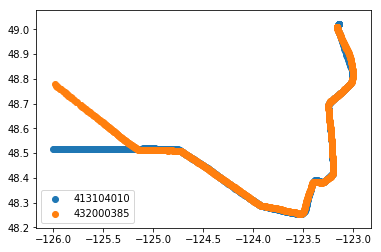
\includegraphics[scale = .8]{figures/VesselRendevouz2d}
    \caption{Two vessel routes}
    \label{fig: VesselRendevouz2d}
\end{figure}

While is obvious that the routes are similar in a positional way, they occur at different times, as is can be see in the figure ~\ref{fig: VesselRendevouz3d} .

\begin{figure}[H]
	\centering
	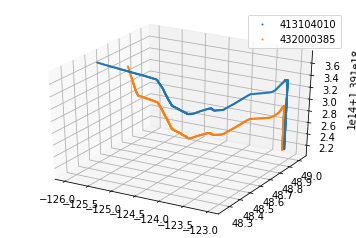
\includegraphics[scale = .9]{figures/VesselRendevouz3d}
    \caption{Two vessel routes, time on Z-axis}
    \label{fig: VesselRendevouz3d}
\end{figure}

%-----------RB-ADS-----------

\section{Rule Based Anomaly Detection Service}
A Rule is defined as something that can, at least in the way we approach them, be expressed as an if-then sentence, \cite{Edlund2006titleRule-basedSurveillance/title}
Anomaly Detection based on the definition of rules, is extremely used in the literature, as it represents an effective way to detect Anomalies at seas. Although this in only viable if and only if the rules are defined by Subject Matter Experts (SMEs) \cite{Boinepalli2014AAlgorithm, Will2011FastProcesses}.

Rule Based Anomaly Detection Service, was developed to detect Anomalies that can be codified into a rule or a set of rules, in real-time. 
Our approach to detect Anomalies in real-time was by storing the $N$ last Behavioural Points for each Vessel in a Service Cache, working like a first in first out (FIFO) queue. $N$ is a configurable Value, which represents the limit of messages stored in Service Cache for each Vessel, we provide an intuitively way to reduce the hardware requirements to run this service in Real-Time.

When the Service Cache has stored $N$ $BPs$ for a certain Vessel the Rule Based Anomaly Service is called for this Vessel, as demonstrated in Figure\ref{fig: RBADS}, in Vessel MMSI n case.
If a Vessel queue has $N$ $BPs$, and was the Rule Based Anomaly Service was already called of this messages, all Vessel Service Cache being FIFO, we discard the oldest $BPs$, thus the Vessel Queue after is full for the first time it as always $N$.

\begin{figure}[H]
	\centering
	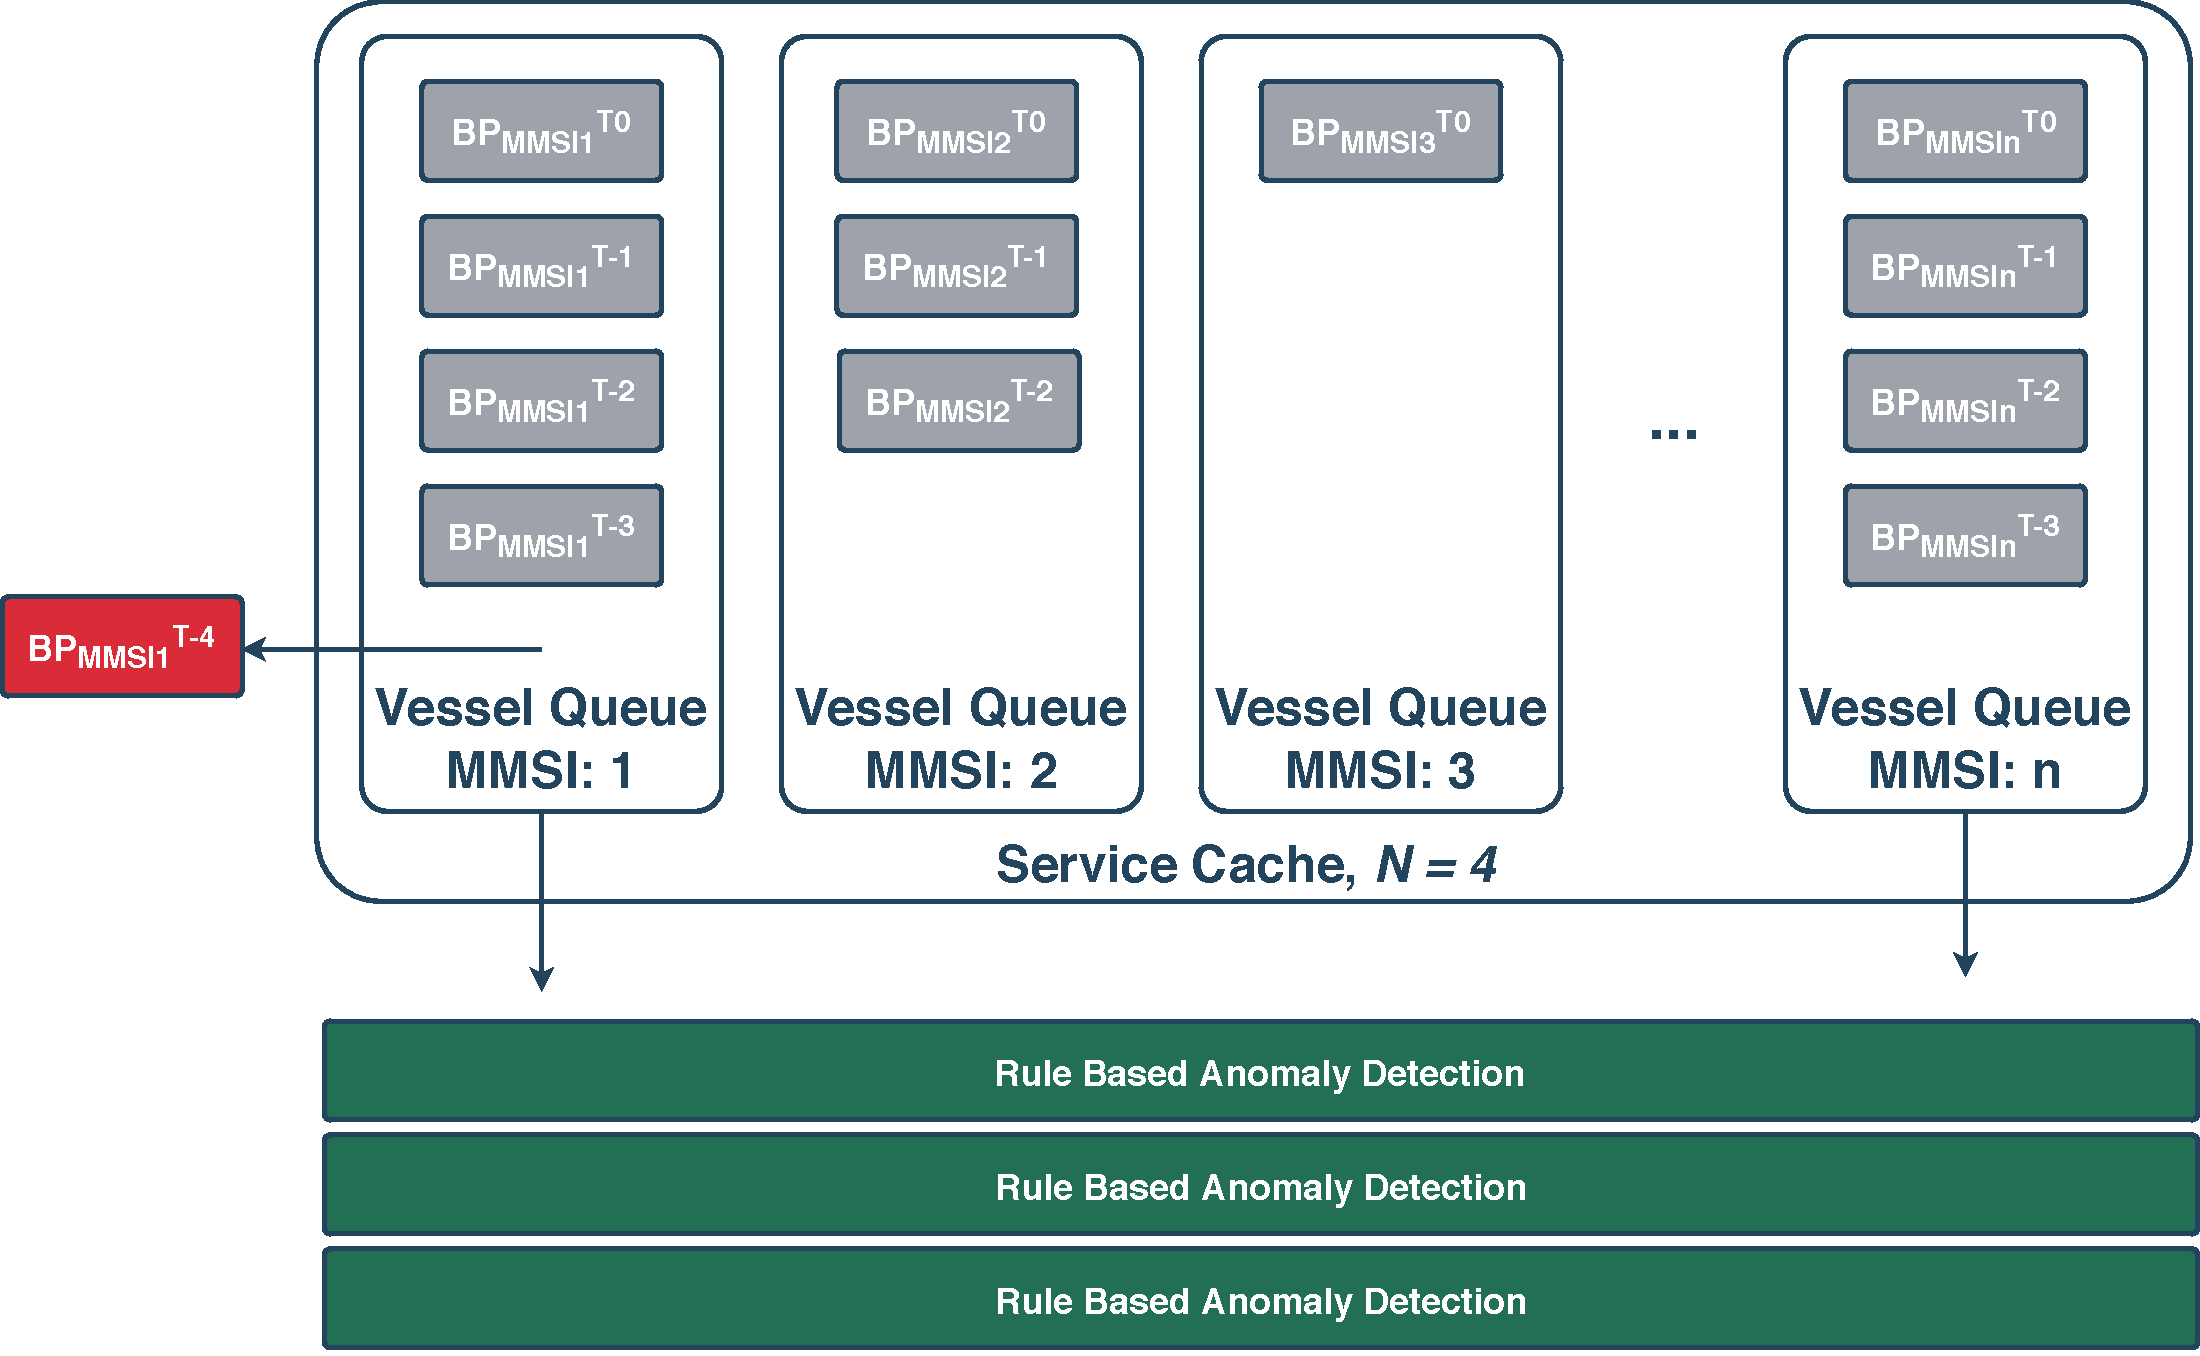
\includegraphics[scale = .36]{figures/Ch4/RBADS.pdf}
    \caption{Demonstration of a possible cases for RBADS Service Cache coordinator.}
    \label{fig: RBADS}
\end{figure}

Rule-Based Anomaly Detection Service, allows a detection of Anomalies based on little previous knowledge of each Vessel Trajectory. Despite the Service could be configured with any Rule that could be written for either Temporal, Spatial or Features based Rules, for example:

\textit{If Vessel MMSI: X in Zone: Y Stopped for more than M minutes then Report as Anomaly.}

For this work we decided to focus on the creation of configurable Rules that could detect the Anomalies presented in Section XX, as were the Anomalies that would be Validated by Maritime Officers,  which we present in Subsections Under.

\subsection{Speed}
Speed represents a Set of configurable Rules that were implemented to detect the Anomaly, $(AR_2)$, defined in Section XX.

Our first approach for the detection of an \textit{Abnormal Change of Velocity} was, calculating the $SoG$ difference from the latest received, $BP^T$ with the previous $BPs^{T-1}$, stored in the Vessel Queue.
If the difference is bigger than a defined $SoG$ $Treshold$, then an Anomaly is generated with the $BPs$ stored in the Message Queue, and the configurations that generated this Anomaly, which could be represented as:
\begin{align*}
\mathbf{if}\;\;& abs({BP_{MMSIn}}^{T}.SoG - {BP_{MMSIn}}^{T-1}.SoG) > SpeedThreshhold
\;\;\mathbf{then} \\ 
&Anomaly[{BP_{MMSIn}}^{T}, {BP_{MMSIn}}^{T-1}] 
\end{align*}
Although, calculating the $SoG$ difference was only viable if  $N = 2 $ was considered as the size of the Vessel Queue.
When considering more than two $BPs$ the difference is not representative of the actual \textit{Abnormal Change of Speed}, in order to mitigate this we created a new configuration, representing the operation it should be done in this case, which for this anomaly we considered the Average Difference, the Max Difference.

\subsection{Course}
Similar the \textbf{Speed} defined above, Course represents a Set of configurable Rules implemented for the Anomaly detection, of $(AR_1)$, which is the \textit{Detection of Abnormal change of Direction}. 
Our approach for the detection of $(AR_1)$ was quite similar to the {Detection abnormal change of Velocity}. 
Although, we noticed depending how Vessels are Moored at port\footnote{http://marineinsight.com/marine-navigation/mooring-methods-ships/}  Vessels tend to swing, due to the Sea Currents, or just from the movement of other Vessels moving in Ports. This creates abrupt changes of $CoG$, which are not representative of the Anomaly Requirement $(AR_1)$.

In order to mitigate this problem, we defined other configurable condition, Minimum SoG Threshold. Thus, the representation of the configurable Set of rules for the detection of rule for the detection of $(AR_1)$, is :

\[If abs(MQ_{T}.CoG - MQ_{T-1}.CoG)  and  MQ_T.SoG > S then Anonalous.\]


\subsection{AIS Signal Loss}
The \textit{disappearance from sensor coverage for more than a configurable Time Period}, $(AR_3)$, can be caused for numerous reason as it is mentioned in Section XX. From a data stand point the disappearance from sensor coverage is represented as the loss of signal, or in other words, the non reception of AIS messages from this Vessel for more than $M$ Minutes.

In this work, we detect the loss of signal from Vessel, by analyzing when did a certain Vessel transmitted for the last time. This is done in real time, by the RBADS by one of two ways: the A priori way or the posteriori way.

First, as we store the Last $N$ $BPs$ for each Vessel that we received AIS messages from, in a the respective Message Queue from the Service Cache. By calculating the difference between the the last received ${BP_{MMSI}}^T$ to the ${BP_{MMSI}}^T-1$, we can know what was the elapsed time. Therefore, if this elapsed Time is bigger than a configurable Time $M$, this is reported as Anomaly. This method is considered a posteriori, as we are waiting for a new message to generate a Signal Loss Anomaly.

The a priori way, is when a Signal Loss anomaly is generated with out the reception of the a new message of a certain Vessel. Having the latest $BP$ for each Vessel stored in the Vessel Queue, if more than $M$ minutes have passed without receiving a Message for this Vessel an anomaly is generated. Both methods of detection represent the actual Signal Loss from a Data Stand point, and depending on the situation both can generate value to the End-Users. 

\iffalse
\section{DUMPZ}

\todo[inline]{this needs to be done...}
Ships equipped with AIS are obliged to keep the AIS autonomously transmitting AIS messages. A way that ships illegally hide their position and possible what the ships is doing objectively, is by switching off the AIS, or finding ways to block the communications of the AIS transmitter with the coastal receivers.

This creates a problem in the maritime domain, has maritime authorities are constantly finding new ways to discover this illegal activities. A method that looks into historical or new streams of data, was developed. 

This method efficiently uses Data Wrangling techniques, in witch with the aid of powerful Python libraries such as Pandas and Data-Frames, the vessels that don't transmit any information for a parametrized time period, are detected and can be reported for maritime authorities for future investigation.

In table ~\ref{Table: AIS signal loss}, results from the above described method are presented, for this work were conducted on a sub-set of the main data-set, that is, from 50 vessel trajectories, which represents 50,000 AIS messages.

\begin{table}[H]
\centering
\caption{Example of the results, obtained for AIS signal loss, with 50 Ships subset.}
\label{Table: AIS signal loss}
\begin{tabular}{@{}lllll@{}}
\toprule
MMSI & X & Y & Time & Signal Loss Time \\ \midrule
316007330 & -125.990797 & 48.867373 & 2014-02-23 21:43:21 & 18 days 13:53:16 \\
316199201 & -123.375432 & 48.430820 & 2014-02-13 12:26:36 & 11 days 08:18:25 \\
338670018 & -121.378175 & 37.977128 & 2014-02-08 20:18:29 & 7 days 20:06:22 \\
367556504 & -122.495912 & 37.869303 & 2014-02-10 20:45:48 & 7 days 01:57:47 \\
... & ... & ... & ... & ... \\
311240050 & -121.781132 & 30.241660 & 2014-02-06 03:15:42 & 0 days 00:18:39 \\
311240012 & -121.725685 & 30.196453 & 2014-02-08 07:34:12 & 0 days 00:08:30 \\ 
\bottomrule
\end{tabular}
\end{table}
for this work we focused on the creation of rules that would detect the anomlies presented in Section XX, which are the Anomalies presented in the subsctions under.  

for this work, were defined based on the Anomalies defined in Section XX, but also the Anomalies that could be detected based on little previous knowledge of the previous Vessel Trajectory. Based on the previous $N$ $BPs$ that the Service Cache, had stored for each Vessel we are able to detect the Anomalies which we defined as: 

\begin{itemize}
  \item Speed -  - 
  \i$ , definec d in Section XX. AS  (AR_2)$tem Course - $(AR_1)$ - 
  \item Signal Loss - $(AR_1)$ - 
\end{itemize}

was developed to detect the Anomalies that could be detected by the 
For this work we focused on the development of rules that can Validate Anomalies, which were presented in Section XX....when decomposed in three topics. 



\todo[inline]{this above is dump...}
only the are receiveis received f

The has 
The $N$ last Behavioural Points stored for each Vessel are then parsed on the Configurable Rules which are completely configurable for this Service. For this Service, we provide  in the Rule-Based ADS are then 

which can limit the ammount of taking a full advantage from the Spark Streaming Data-Frames and Kafka funcionalities.

Despite being possible to create a fully configurable Service that would manage rules, and 

From the anomalies defined in Sec. XX, and by accessing Maritime Expert Knowledge via the MARISA project, we concluded that, apart from the Anomalies detected by the Anomaly Detection Service (Sec. XX), 
\fi



